\chapter[Experimentos y resultados]{Experimentos y resultados}
\label{ch:exp_result}

\section{Base de datos MMI}
\label{exp:bdd}
Para poder realizar los experimentos con el algoritmo propuesto en el Capítulo~\ref{ch:algoritmo}, se utilizo una base de datos preparada para el reconocimiento facial y de expresiones faciales. Creada por Pantic \etal~\cite{Pantic2005}, MMI es una base de datos multiuso que en esta instancia se utilizo para el reconocimiento de expresiones faciales. Contiene mas de 1000 ejemplos clasificados tanto en imágenes como vídeos; 19 sujetos de prueba; Las edades de los sujetos de prueba varían entre los 19 y los 62 años;  contiene tanto hombres como mujeres, además de tres razas étnicas distintas; Y por ultimo tanto las imágenes como los vídeos están grabados de forma frontal y lateral con respecto al rostro del sujeto. En esta ocasión utilizamos los vídeos grabados de forma frontal, y siendo cada uno de estos etiquetado con una clase distinta para cada expresión facial: Ira(1), Asco(2), Miedo(3), Alegría(4), Tristeza(5) y Sorpresa(6).

\section{Experimentos}
\label{exp:exp}

Para poder probar la efectividad y buen modelado del algoritmo propuesto en el Capítulo~\ref{ch:algoritmo}, se preparo una pila de experimentos, los cuales permitieron realizar una revisión del modelado y precisión de método.
Se prepararon pruebas para cada uno de los pasos del algoritmo, las cuales nos permitieron elegir los mejores valores para cada una de las variables a utilizar.

Para la etapa de Extracción de micro-descriptores propuesta en la Sección~\ref{algoritmo:ext_rayos}, se realizaron pruebas que permitieron ver el modelado de los \textit{rayos de flujo} con respecto al movimiento de los pixeles a lo largo de los vídeos, y la elección del tamaño de la Región de soporte $R$ y la Ventana de búsqueda $W$.

En la etapa de Normalización de micro-descriptores, propuesto en la Sección~\ref{algoritmo:normalizacion}, se realizaron pruebas con distintos tamaños de $N$ (Variable utilizada para describir el nuevo tamaño de los \textit{rayos de flujo}) y se realizaron comparaciones con respecto a la Asertividad (Accuracy en ingles) de cada valor.

Para la creación de macro-descriptores, propuesta en la Sección~\ref{sec:macro-descriptores}, se prepararon dos experimentos distintos, primero se realizo un estudio del agrupamiento de los \textit{rayos} en el rostro para cada uno de los vídeos con distintos valores $K$, el cual indica la cantidad de grupos de \textit{rayos de flujo} existen y como se distribuyen en el rostro; el segundo experimento que se realizó fue calcular la Asertividad (Accuracy en ingles) para distintos valores de la variable $K$.

Por ultimo en la etapa de entrenamiento y posterior clasificación, explicada en la Sección~\ref{sec:clasificacion}, se realizaron pruebas con los distintos \textit{Kernel} y sus respectivas variables, los cuales son recibidos por SVM para la generación del modelo.


\subsection{Extracción de micro-descriptores}
\label{exp:micro-descriptores}

Etapa propuesta en al Sección~\ref{algoritmo:ext_rayos}, en simples palabras consiste en modelar el movimiento de cada uno de los pixeles a lo largo de todo el vídeo, este modelado es llamado \textit{rayo de flujo}. Para poder extraer un \textit{rayo} se utilizan dos ventanas: la región de soporte y la ventana de búsqueda. Estas regiones permiten calcular a que pixel $(x',y')$ en un tiempo $t+1$ se desplazo pixel $(x,y)$ en un tiempo $t$. Luego de calcular el movimiento de un pixel de $t$ a $t+1$ se crea un \textit{rayo de soporte}, que es la composición mínima para la creación de los \textit{rayos de flujo}.



\definecolor{lightgray}{gray}{0.9}
\begin{table}[t!]
	\centering
	\begin{tabular}{ |>{\centering\arraybackslash}m{2cm} | >{\centering\arraybackslash}m{2cm} | >{\centering\arraybackslash}m{1.5cm} | >{\centering\arraybackslash}m{1.5cm} | >{\centering\arraybackslash}m{2cm} | >{\centering\arraybackslash}m{1.5cm} | >{\centering\arraybackslash}m{1.5cm} | }
		\hline
		Expresión & \multicolumn{3}{| c |}{Imágenes sin codificación} & \multicolumn{3}{| c |}{Imágenes con LBP}\\
		\hline
		& Imagen & XT & YT & Imagen & XT & YT \\
		(E1) \ \ \ \ \ \ Ira & 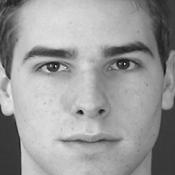
\includegraphics[height=2cm]{Figuras/resultados/E1/E1.png} & 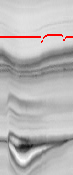
\includegraphics[height=2cm]{Figuras/resultados/E1/E1_YT.png} & 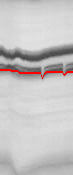
\includegraphics[height=2cm]{Figuras/resultados/E1/E1_XT.png} & 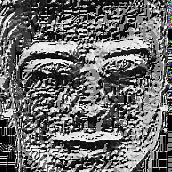
\includegraphics[height=2cm]{Figuras/resultados/E1/E1_LBP.png} & 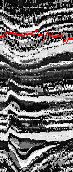
\includegraphics[height=2cm]{Figuras/resultados/E1/E1_LBP_YT.png} & 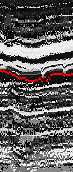
\includegraphics[height=2cm]{Figuras/resultados/E1/E1_LBP_XT.png} \\
		
		(E2) \ \ \ \ Asco& 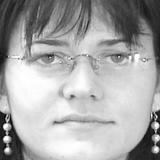
\includegraphics[height=2cm]{Figuras/resultados/E2/E2.png} & 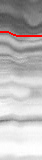
\includegraphics[height=2cm]{Figuras/resultados/E2/E2_YT.png} & 
\includegraphics[height=2cm]{Figuras/resultados/E2/E2_XT.png} & 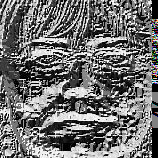
\includegraphics[height=2cm]{Figuras/resultados/E2/E2_LBP.png} & 
\includegraphics[height=2cm]{Figuras/resultados/E2/E2_LBP_YT.png} & 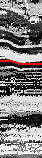
\includegraphics[height=2cm]{Figuras/resultados/E2/E2_LBP_XT.png} \\
		
		(E3) \ \ \ \ Miedo& 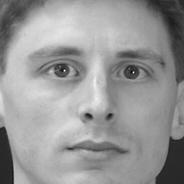
\includegraphics[height=2cm]{Figuras/resultados/E3/E3.png} & 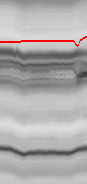
\includegraphics[height=2cm]{Figuras/resultados/E3/E3_YT.png} & 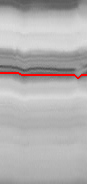
\includegraphics[height=2cm]{Figuras/resultados/E3/E3_XT.png} & 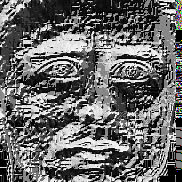
\includegraphics[height=2cm]{Figuras/resultados/E3/E3_LBP.png} & 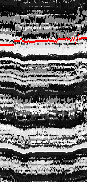
\includegraphics[height=2cm]{Figuras/resultados/E3/E3_LBP_YT.png} & 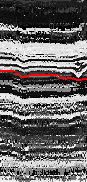
\includegraphics[height=2cm]{Figuras/resultados/E3/E3_LBP_XT.png} \\
		
		(E4) Alegría & 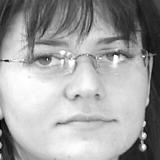
\includegraphics[height=2cm]{Figuras/resultados/E4/E4.png} & 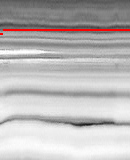
\includegraphics[height=2cm]{Figuras/resultados/E4/E4_YT.png} & 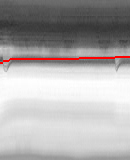
\includegraphics[height=2cm]{Figuras/resultados/E4/E4_XT.png} & 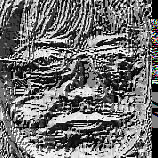
\includegraphics[height=2cm]{Figuras/resultados/E4/E4_LBP.png} & 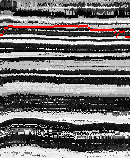
\includegraphics[height=2cm]{Figuras/resultados/E4/E4_LBP_YT.png} & 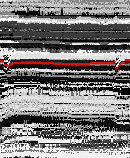
\includegraphics[height=2cm]{Figuras/resultados/E4/E4_LBP_XT.png} \\
		
		(E5) Tristeza& 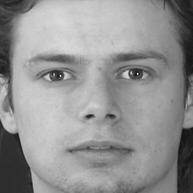
\includegraphics[height=2cm]{Figuras/resultados/E5/E5.png} & 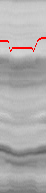
\includegraphics[height=2cm]{Figuras/resultados/E5/E5_YT.png} & 
\includegraphics[height=2cm]{Figuras/resultados/E5/E5_XT.png} & 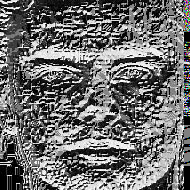
\includegraphics[height=2cm]{Figuras/resultados/E5/E5_LBP.png} & 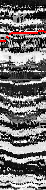
\includegraphics[height=2cm]{Figuras/resultados/E5/E5_LBP_YT.png} & 
\includegraphics[height=2cm]{Figuras/resultados/E5/E5_LBP_XT.png} \\
		
		(E6) Sorpresa& 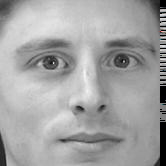
\includegraphics[height=2cm]{Figuras/resultados/E6/E6.png} & 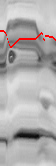
\includegraphics[height=2cm]{Figuras/resultados/E6/E6_YT.png} & 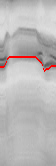
\includegraphics[height=2cm]{Figuras/resultados/E6/E6_XT.png} & 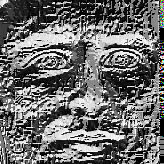
\includegraphics[height=2cm]{Figuras/resultados/E6/E6_LBP.png} & 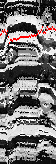
\includegraphics[height=2cm]{Figuras/resultados/E6/E6_LBP_YT.png} & 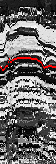
\includegraphics[height=2cm]{Figuras/resultados/E6/E6_LBP_XT.png} \\
		\hline
		
		& (a) & (b) & (c) & (d) & (e) & (f)\\
		\hline
		
	\end{tabular}
	\caption{Tabla comparativa de la extracción de micro-decriptores con vídeos codificados con LBP y sin codificar. Cada fila representa una expresión facial distinta. Las columnas (a) y (d) son el primer cuadro del vídeo, (b) y (e) representan el plano XT, y (c) y (f) representan el plano YT. }
	\label{tabla:comparacion_rayos}
\end{table}


% % % % % % % % % % % % % % % % % % % % % % % % % % % % % % % % % % % % % % % % % % % % % % % % % % % %
% % % % % % % % % % % % % % % % % % % % B O R R A R % % % % % % % % % % % % % % % % % % % % % % % % % %
% % % % % % % % % % % % % % % % % % % % % % % % % % % % % % % % % % % % % % % % % % % % % % % % % % % % 
\subsection{Modelado del movimiento de los pixeles}
\label{exp:rayos}
Para poder probar la existencia de un real modelado del movimiento de los pixeles por parte de los \textit{rayos de flujo}, se creo un programa que recibe como entrada un video y el conjunto de pixeles a analizar su movimiento durante el video. Para esto se utilizo el algoritmo de creación de micro-descriptores analizado de la sección~\ref{sec:micro-_descriptores}. Luego de obtener los \textit{rayos}, se procedio a crear una imagen en los planos $XT$ e $YT$, cada uno de los cuales muestra el desplazamiento de un pixel a los largo del tiempo sobre un eje especifico $x$ e $y$ respectivamente.  

mientras mas grande la diferencia entre la RS y WS mayor es el error a la hora de moverse, por lo cual los rayos tienden a perderse.
con ventanas RS de tamaño 3 funciona bien con 5 y 7 de WS
con ventanas de rs tamaño 5 funciona bien con 7 y 9
con ventanas de rs tamaño 7 funciona bien con 11 y 13

Hablar de que con LBP se pierde los rayos

Mostrar graficos de movimiento en XT e YT
HABLAR DEL COMPORTAMIENTO DE LOS EJES, que el eje x modela, y el eje Y tiende a perderse.
Hablar de experimentos solo en el eje Y


\subsection{Obtencion del Kernel optimo para SVM}

Hablar sobre lo que se realizo para obtener los mejores valores.

Valores obtenidos para LINEAL y mostrar cuadro y grafico de la variable C v/s Accuracy
Valores obtenidos para RBF y mostrar cuadro y grafico para variable Gamma, C y Accuracy
valores obtenidos para Sigmoid y mostrar cuado de grafico para sus variables
valores obtenidos para Poly y mostrar cuajdro de graficos para sus variables

Hablar de Kernels para Histogramas y hablar de valores obtenidos con el kernel de comparacion de histograma


\subsection{Pruebas sobre variables del algoritmo}
\label{exp:var}
Como se explica en el Capítulo~\ref{ch:algoritmo}, el algoritmo cuenta con tres variables importantes, las cuales son la clave para la eficacia y precisión de este. Estas variables son el tamaño de la \textit{región de soporte} o variable $L$, el valor de la normalización de los \textit{rayos de soporte} o variable $N$ y por ultimo el tamaño del \textit{Bag of Visual Words} o variable $K$.

\subsubsection{Pruebas del tamaño de la región de soporte}
Como se explica en la Sección~\ref{algoritmo:ext_rayos}, la extracción de \textit{rayos}, se utilizan dos estructuras llamadas \textit{región de soporte} y \textit{ventana de búsqueda}, estas son de tamaño $L$x$L$ y $(2L+1)$x$(2L+1)$ respectivamente. El valor de la variable $L$ es muy importante ya que define el tamaño de ambas regiones, y a su vez permite definir el tamaño de la región donde se busca el movimiento de los píxeles, por lo cual un gran tamaño puede indicar mayor precisión y a su vez menor velocidad. La idea de estas pruebas es poder encontrar el valor óptimo de $L$ el cual permita tener una respuesta aceptable por parte del algoritmo. 

\subsubsection{Pruebas de normalización de rayos}	

La normalización de rayos, explicada en la Sección~\ref{algoritmo:normalizacion}, es otro de los procesos a los cuales se debe encontrar un valor óptimo a su variable $N$, esta variable indica cual debe ser el largo de los vectores que representan los \textit{rayos} de los vídeos. El proceso de normalización es un proceso en el cual se requiere llevar todos los vectores al mismo espacio vectorial, para así poder realizar comparaciones entre estos. Este proceso tiene una gran desventaja, esto debido a que al transformar un vector de tamaño mayor a $N$ este tiende a perder información en su compresión, al igual que al agrandar un vector de tamaño menor a $N$ se tiende a agregar información que posiblemente sea falsa o simplemente ruido.

\subsubsection{Pruebas del tamaño del \textit{Bag of Visual Words}}
La técnica de \textit{Bag of Visual Words} utiliza la variable $K$, está representa el numero de \textit{clusters} o grupos que se deben formar en el proceso de creación de la bolsa de palabras, a su vez también indica el tamaño del descriptor final o macro-descriptor que representa a cada vídeo. Esta variable es la  más importante en el algoritmo, esto debido a que una mala elección de la cantidad de \textit{clusters}, puede desencadenar en una mala creación de los macro-descriptores, por lo cual la búsqueda del valor óptimo es muy importante para obtener una buena precisión. La única forma de poder encontrar un valor óptimo o funcional es a través del método de prueba y error, esto debido a que no existe una forma empírica de demostrar cual es el valor óptimo para cada corrida.



\subsection{Pruebas codificando los vídeos}
\label{exp:cod}
En la sección~\ref{sec:micro_descriptores}, extracción de micro-descriptores, se explica que antes de poder obtener los \textit{rayos} es necesario realizar un proceso de codificación sobre las imágenes, esto pudiendo ayudar a la extracción de los descriptores. Para esto se preparan tres pruebas distintas, en las cuales se utilizan distintas técnicas de codificación.

	\subsubsection{Sin codificación}
	Esta prueba consiste en ver la eficiencia del descriptor encontrado al final del proceso del algoritmo sin utilizar ningún tipo de codificación sobre los valores de los píxeles, por lo cual el proceso de extracción de rayos se realiza sobre el valor de la intensidad de cada imagen.

	\subsubsection{Codificación de LBP}
	Esta prueba consiste en ver la eficacia del descriptor encontrado al final del proceso del algoritmo propuesto, utilizando el proceso de codificación LBP explicado en la Sección~\ref{sec:lbp}. Esta codificación permite que los nuevos valores obtenidos para los píxeles estén relacionados directamente con la vecindad mas cercana, por lo cual esto permitiría poder realizar una mejor extracción de rayos.
